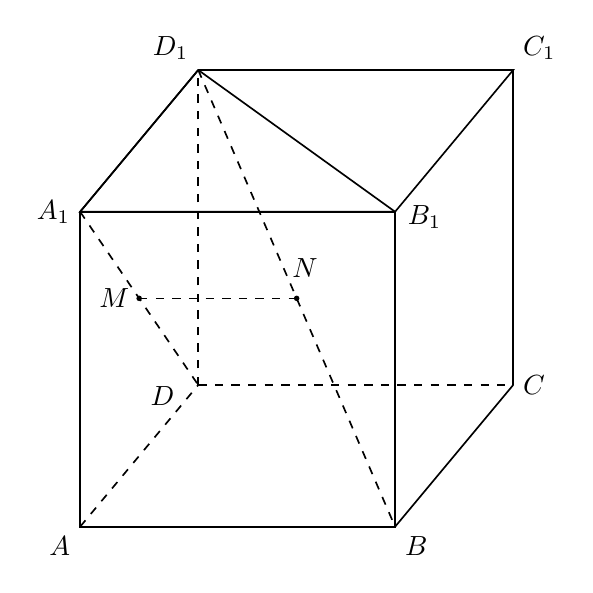
\begin{tikzpicture}[line width=0.6pt, font=\normalsize]
\coordinate (A) at (0,0);
\coordinate (B) at (4,0);
\coordinate (B1) at (4,4);
\coordinate (A1) at (0,4);
\coordinate (D) at (1.5,1.8);
\coordinate (C) at (5.5,1.8);
\coordinate (D1) at (1.5,5.8);
\coordinate (C1) at (5.5,5.8);
\coordinate (M) at (0.75,2.9);
\coordinate (N) at (2.75,2.9);
% front face
\draw (A) -- (B) -- (B1) -- (A1) -- cycle;
% top face
\draw (A1) -- (B1) -- (C1) -- (D1) -- cycle;
% verticals / depth
\draw (B) -- (C);
\draw (C) -- (C1);
\draw (A1) -- (D1);
\draw[dashed] (A) -- (D);
\draw[dashed] (D) -- (C);
\draw[dashed] (D) -- (D1);
% face diagonal A1-D with M
\draw[dashed] (A1) -- (D);
% space diagonal D1-B with N
\draw[dashed] (D1) -- (B);
% top diagonal D1-B1
\draw (D1) -- (B1);
% bottom diagonal D-B

% mid segment M-N
\draw[dashed] (M) -- (N);
\fill (M) circle (1pt);
\fill (N) circle (1pt);
\node[below left] at (A) {$A$};
\node[below right] at (B) {$B$};
\node[left] at (A1) {$A_{1}$};
\node[right,xshift=1.0pt,yshift=-2pt] at (B1) {$B_{1}$};
\node[below left,xshift=-5pt,yshift=3pt] at (D) {$D$};
\node[right] at (C) {$C$};
\node[above left] at (D1) {$D_{1}$};
\node[above right] at (C1) {$C_{1}$};
\node[left] at (M) {$M$};
\node[above,xshift=3pt,yshift=4pt] at (N) {$N$};
\end{tikzpicture}
